\documentclass{standalone}
\usepackage{tikz}
\usetikzlibrary{positioning}

\begin{document}

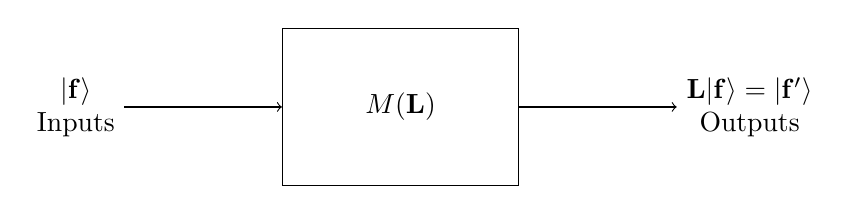
\begin{tikzpicture}[node distance=2cm, every node/.style={align=center}]
    % Input node
    \node (input) {$\vert \mathbf{f} \rangle$ \\ Inputs};
    
    % Machine node
    \node[draw, rectangle, minimum width=3cm, minimum height=2cm, right=of input] (machine) {$M(\mathbf{L})$};
    
    % Output node
    \node[right=of machine] (output) {$\mathbf{L} \vert \mathbf{f} \rangle = \vert \mathbf{f}' \rangle$ \\ Outputs};
    
    % Connect nodes with arrows
    \draw[->] (input) -- (machine);
    \draw[->] (machine) -- (output);
\end{tikzpicture}

\end{document}